\documentclass{article}
\usepackage{graphicx}
\usepackage{tabularx}
\usepackage[landscape, top=2 in, bottom=0.2 in, left=0.2 in, right=0.2 in, papersize={21.59 cm, 27.94 cm}]{geometry}
\usepackage[export]{adjustbox}
\usepackage{fancyhdr}
\usepackage{lastpage}
\usepackage{datetime}
\usepackage{multirow}
\pagestyle{fancy}
\fancyhf{}
\renewcommand{\headrulewidth}{0pt}
\fancyhead[C]{\\ 
\begin{tabular}{ccc}
\multirow{2}{*}{
\includegraphics[width=3cm]{Gold Logo Black Text Transparent.png}} & Vibration Assessment Centrifuges & Rev 0 \\
 & \today & \\
 \end{tabular}}
\begin{document}
\begin{center}
\begin{tabular*}{0.6\textwidth}{@{\extracolsep{\fill}}cc}
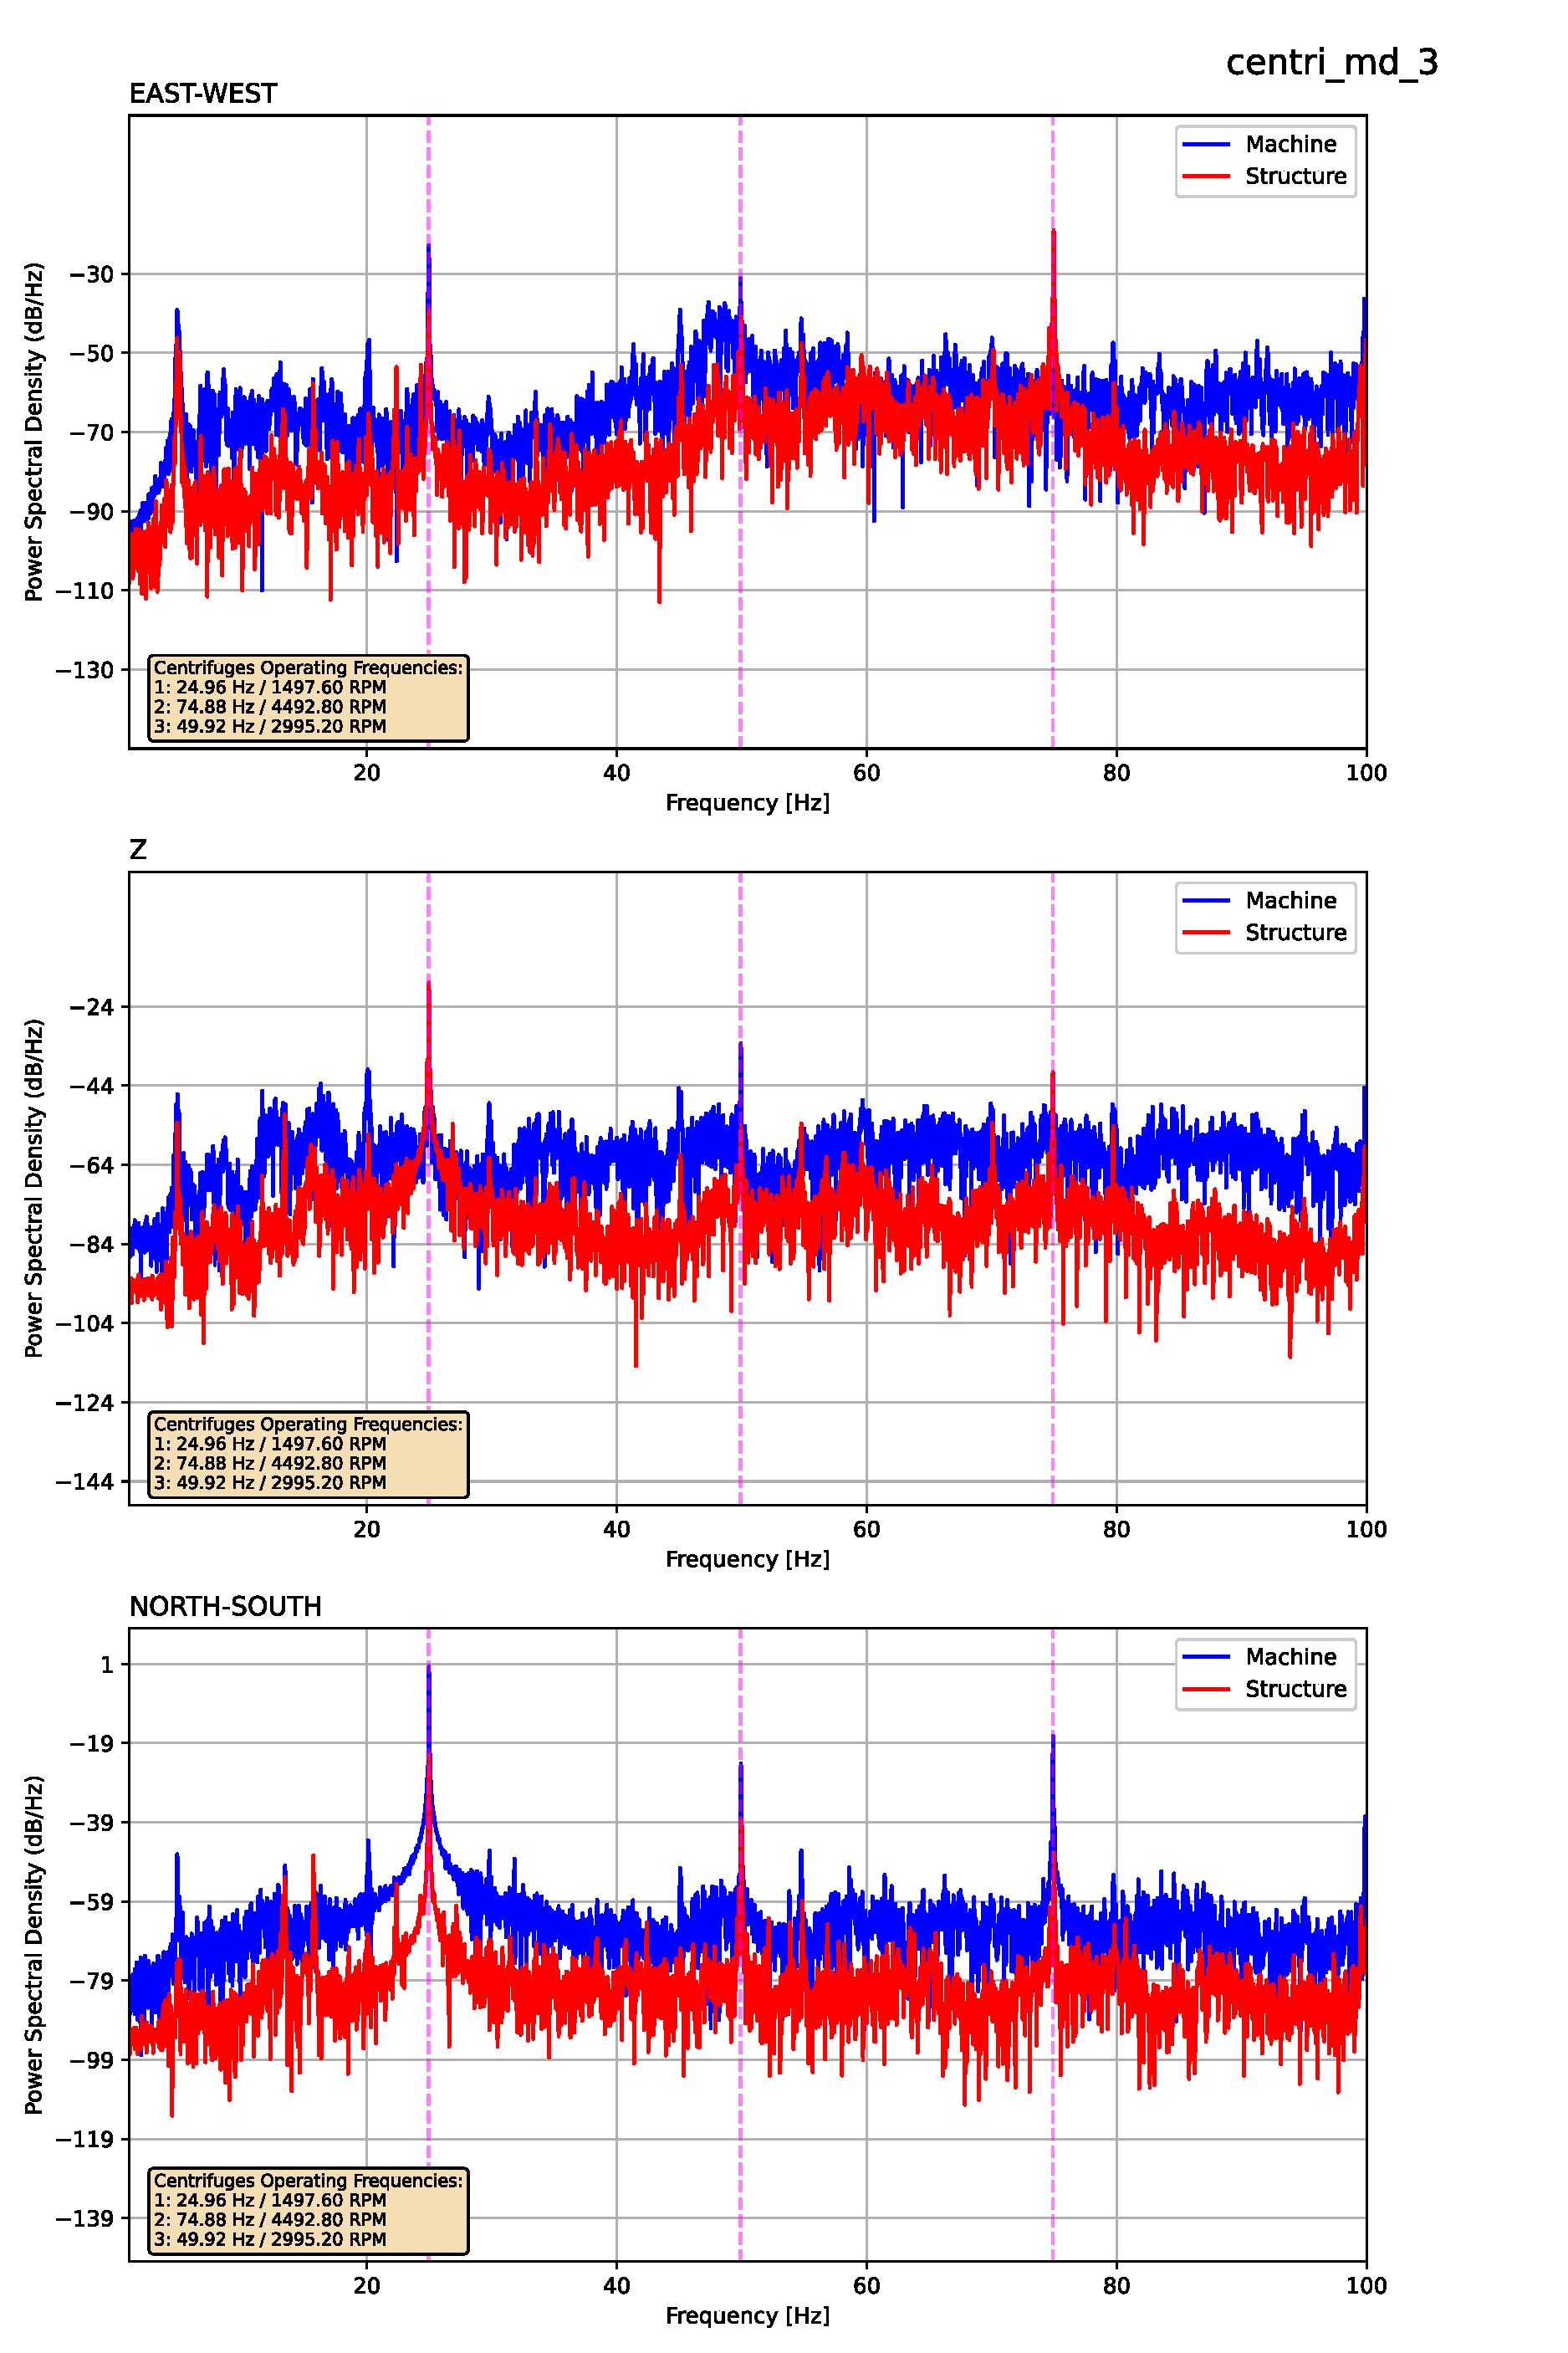
\includegraphics[width=0.3\linewidth, valign=c]{./centri_md_3_comparison.pdf} &
\includegraphics[width=0.3\linewidth, valign=c]{./centri_photos/mod3.JPG} \\
\multicolumn{2}{|p{0.6\textwidth}|}{A vibration assessment was carried out in the following centrifuges measuring acceleration above the vibration dampers and in the supporting structure (after the vibration dampers), the following frequencies were identified: [24.96 74.88 49.92] Hz.
} \\
\end{tabular*}
\end{center}
\newpage
\begin{center}
\begin{tabular*}{0.6\textwidth}{@{\extracolsep{\fill}}cc}
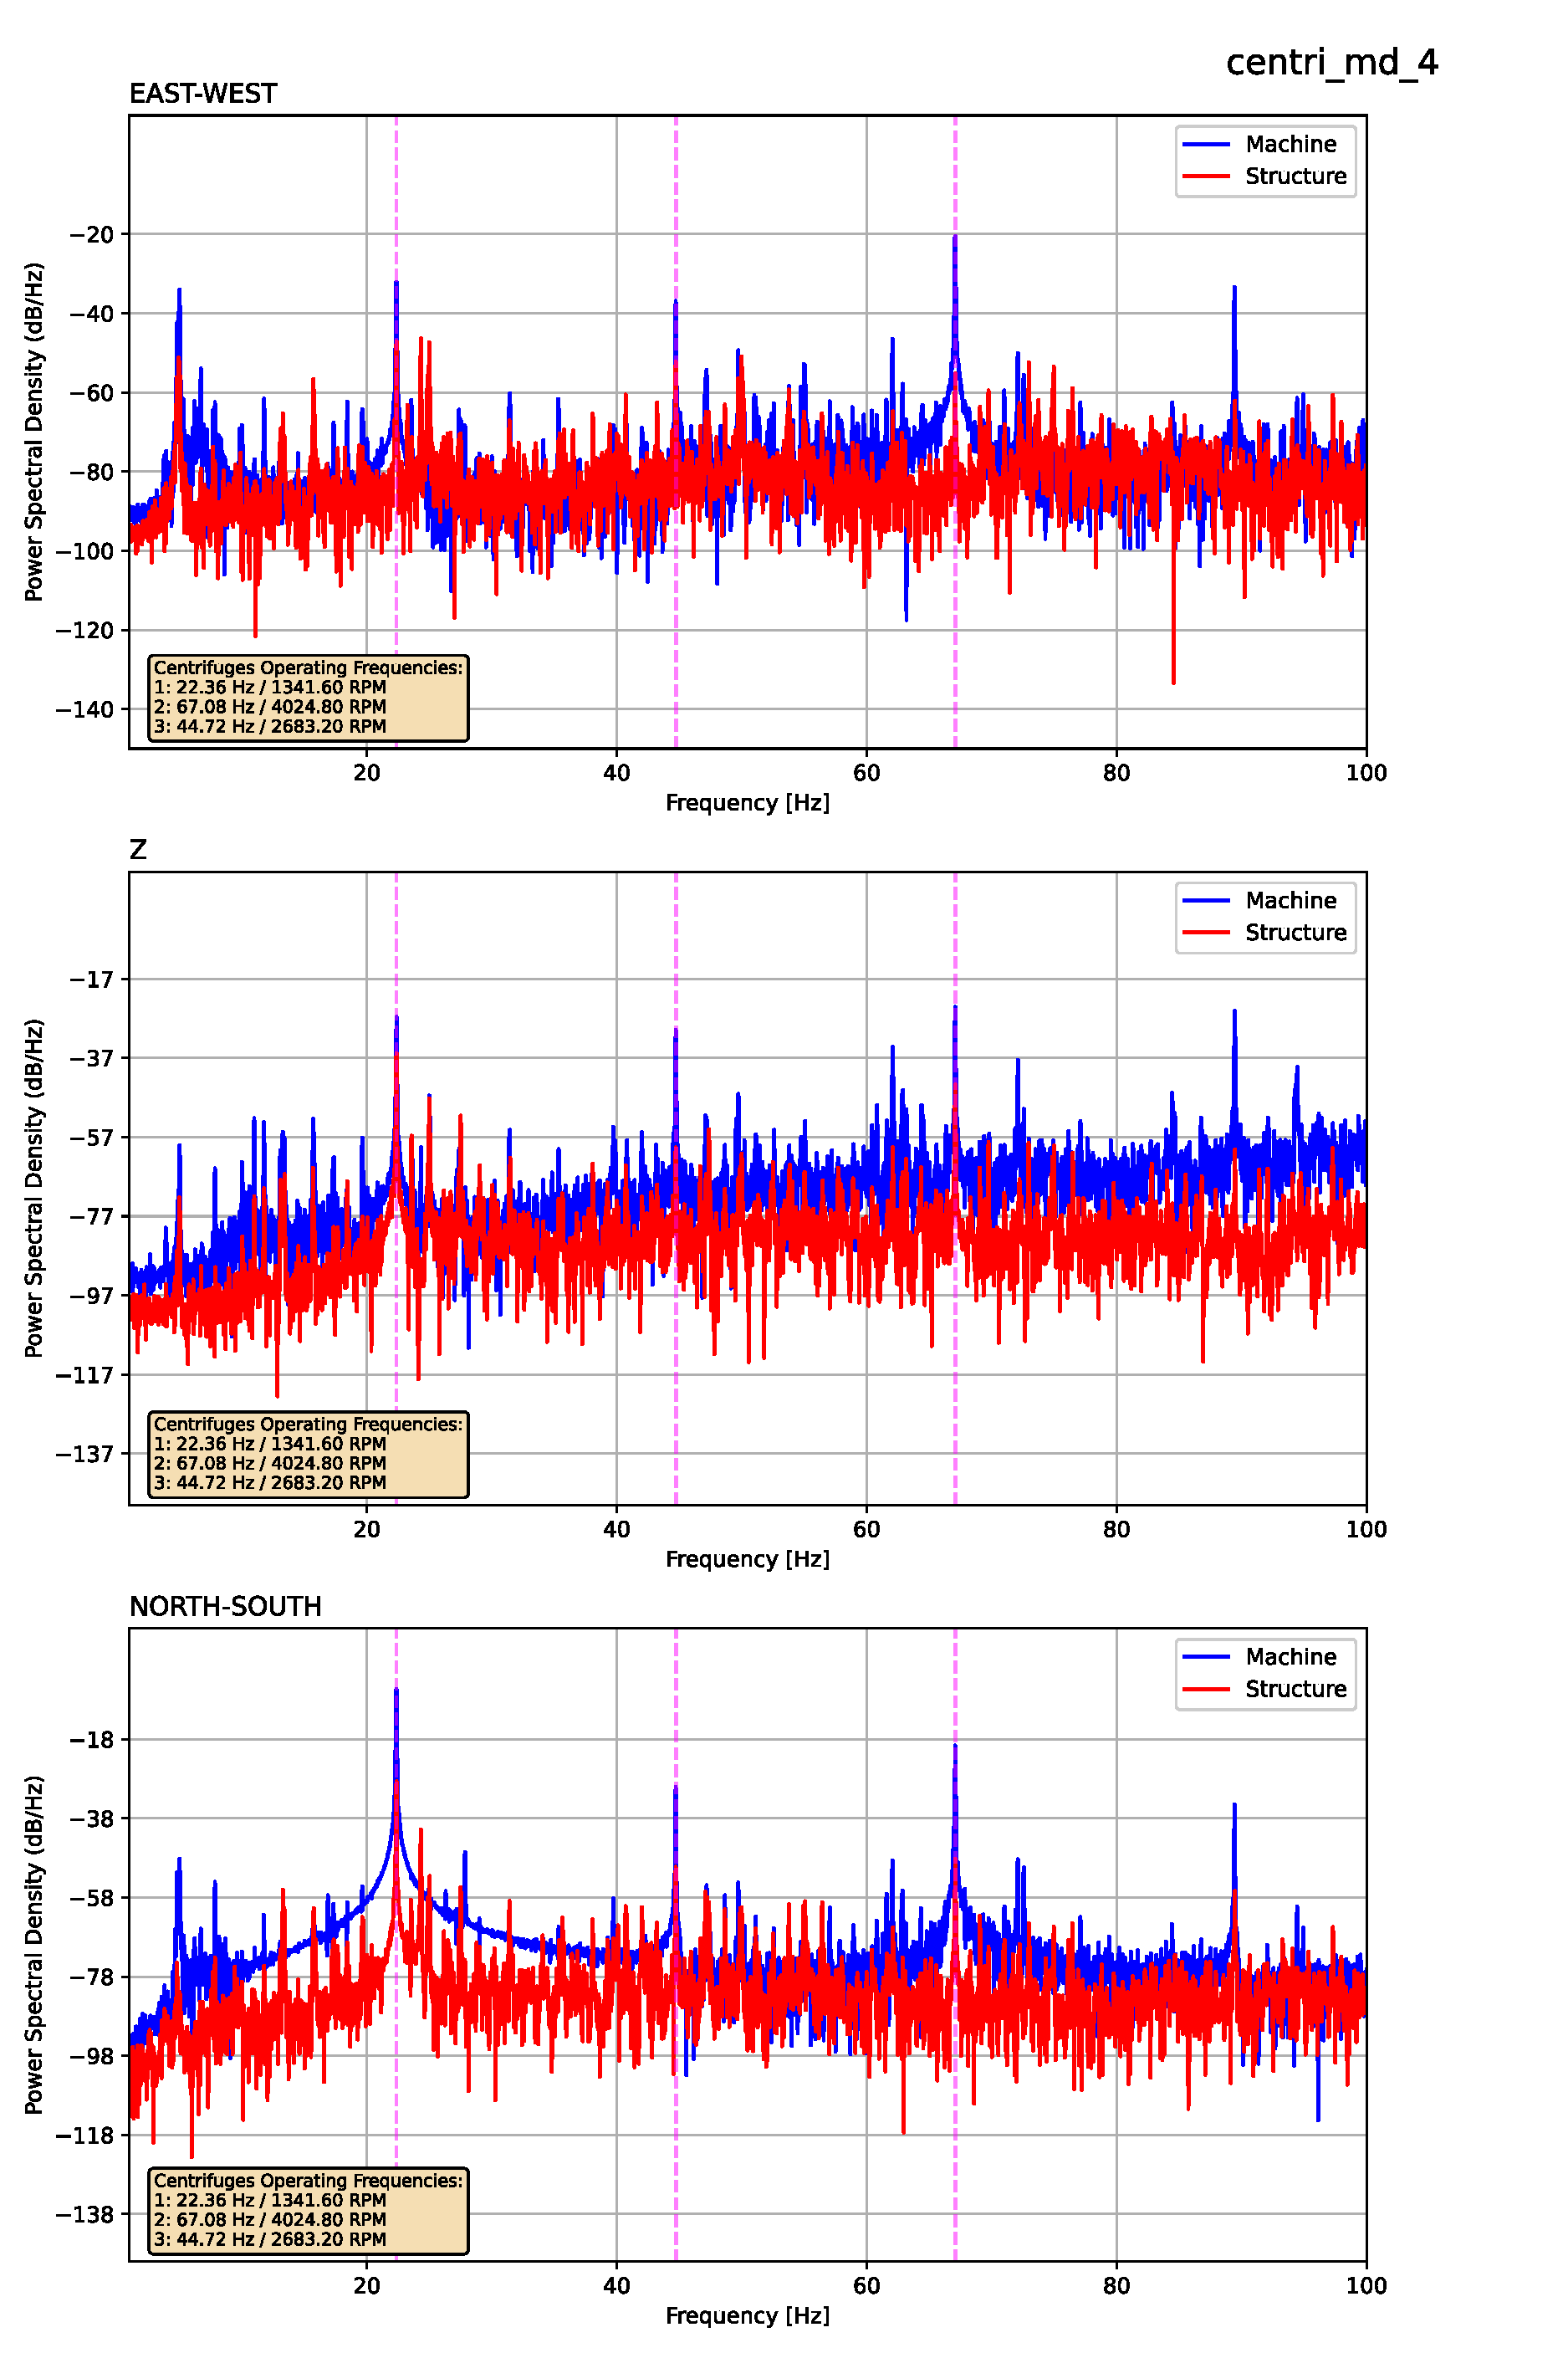
\includegraphics[width=0.3\linewidth, valign=c]{./centri_md_4_comparison.pdf} &
\includegraphics[width=0.3\linewidth, valign=c]{./centri_photos/mod4.JPG} \\
\multicolumn{2}{|p{0.6\textwidth}|}{A vibration assessment was carried out in the following centrifuges measuring acceleration above the vibration dampers and in the supporting structure (after the vibration dampers), the following frequencies were identified: [22.36 67.08 44.72] Hz.
} \\
\end{tabular*}
\end{center}
\newpage
\begin{center}
\begin{tabular*}{0.6\textwidth}{@{\extracolsep{\fill}}cc}
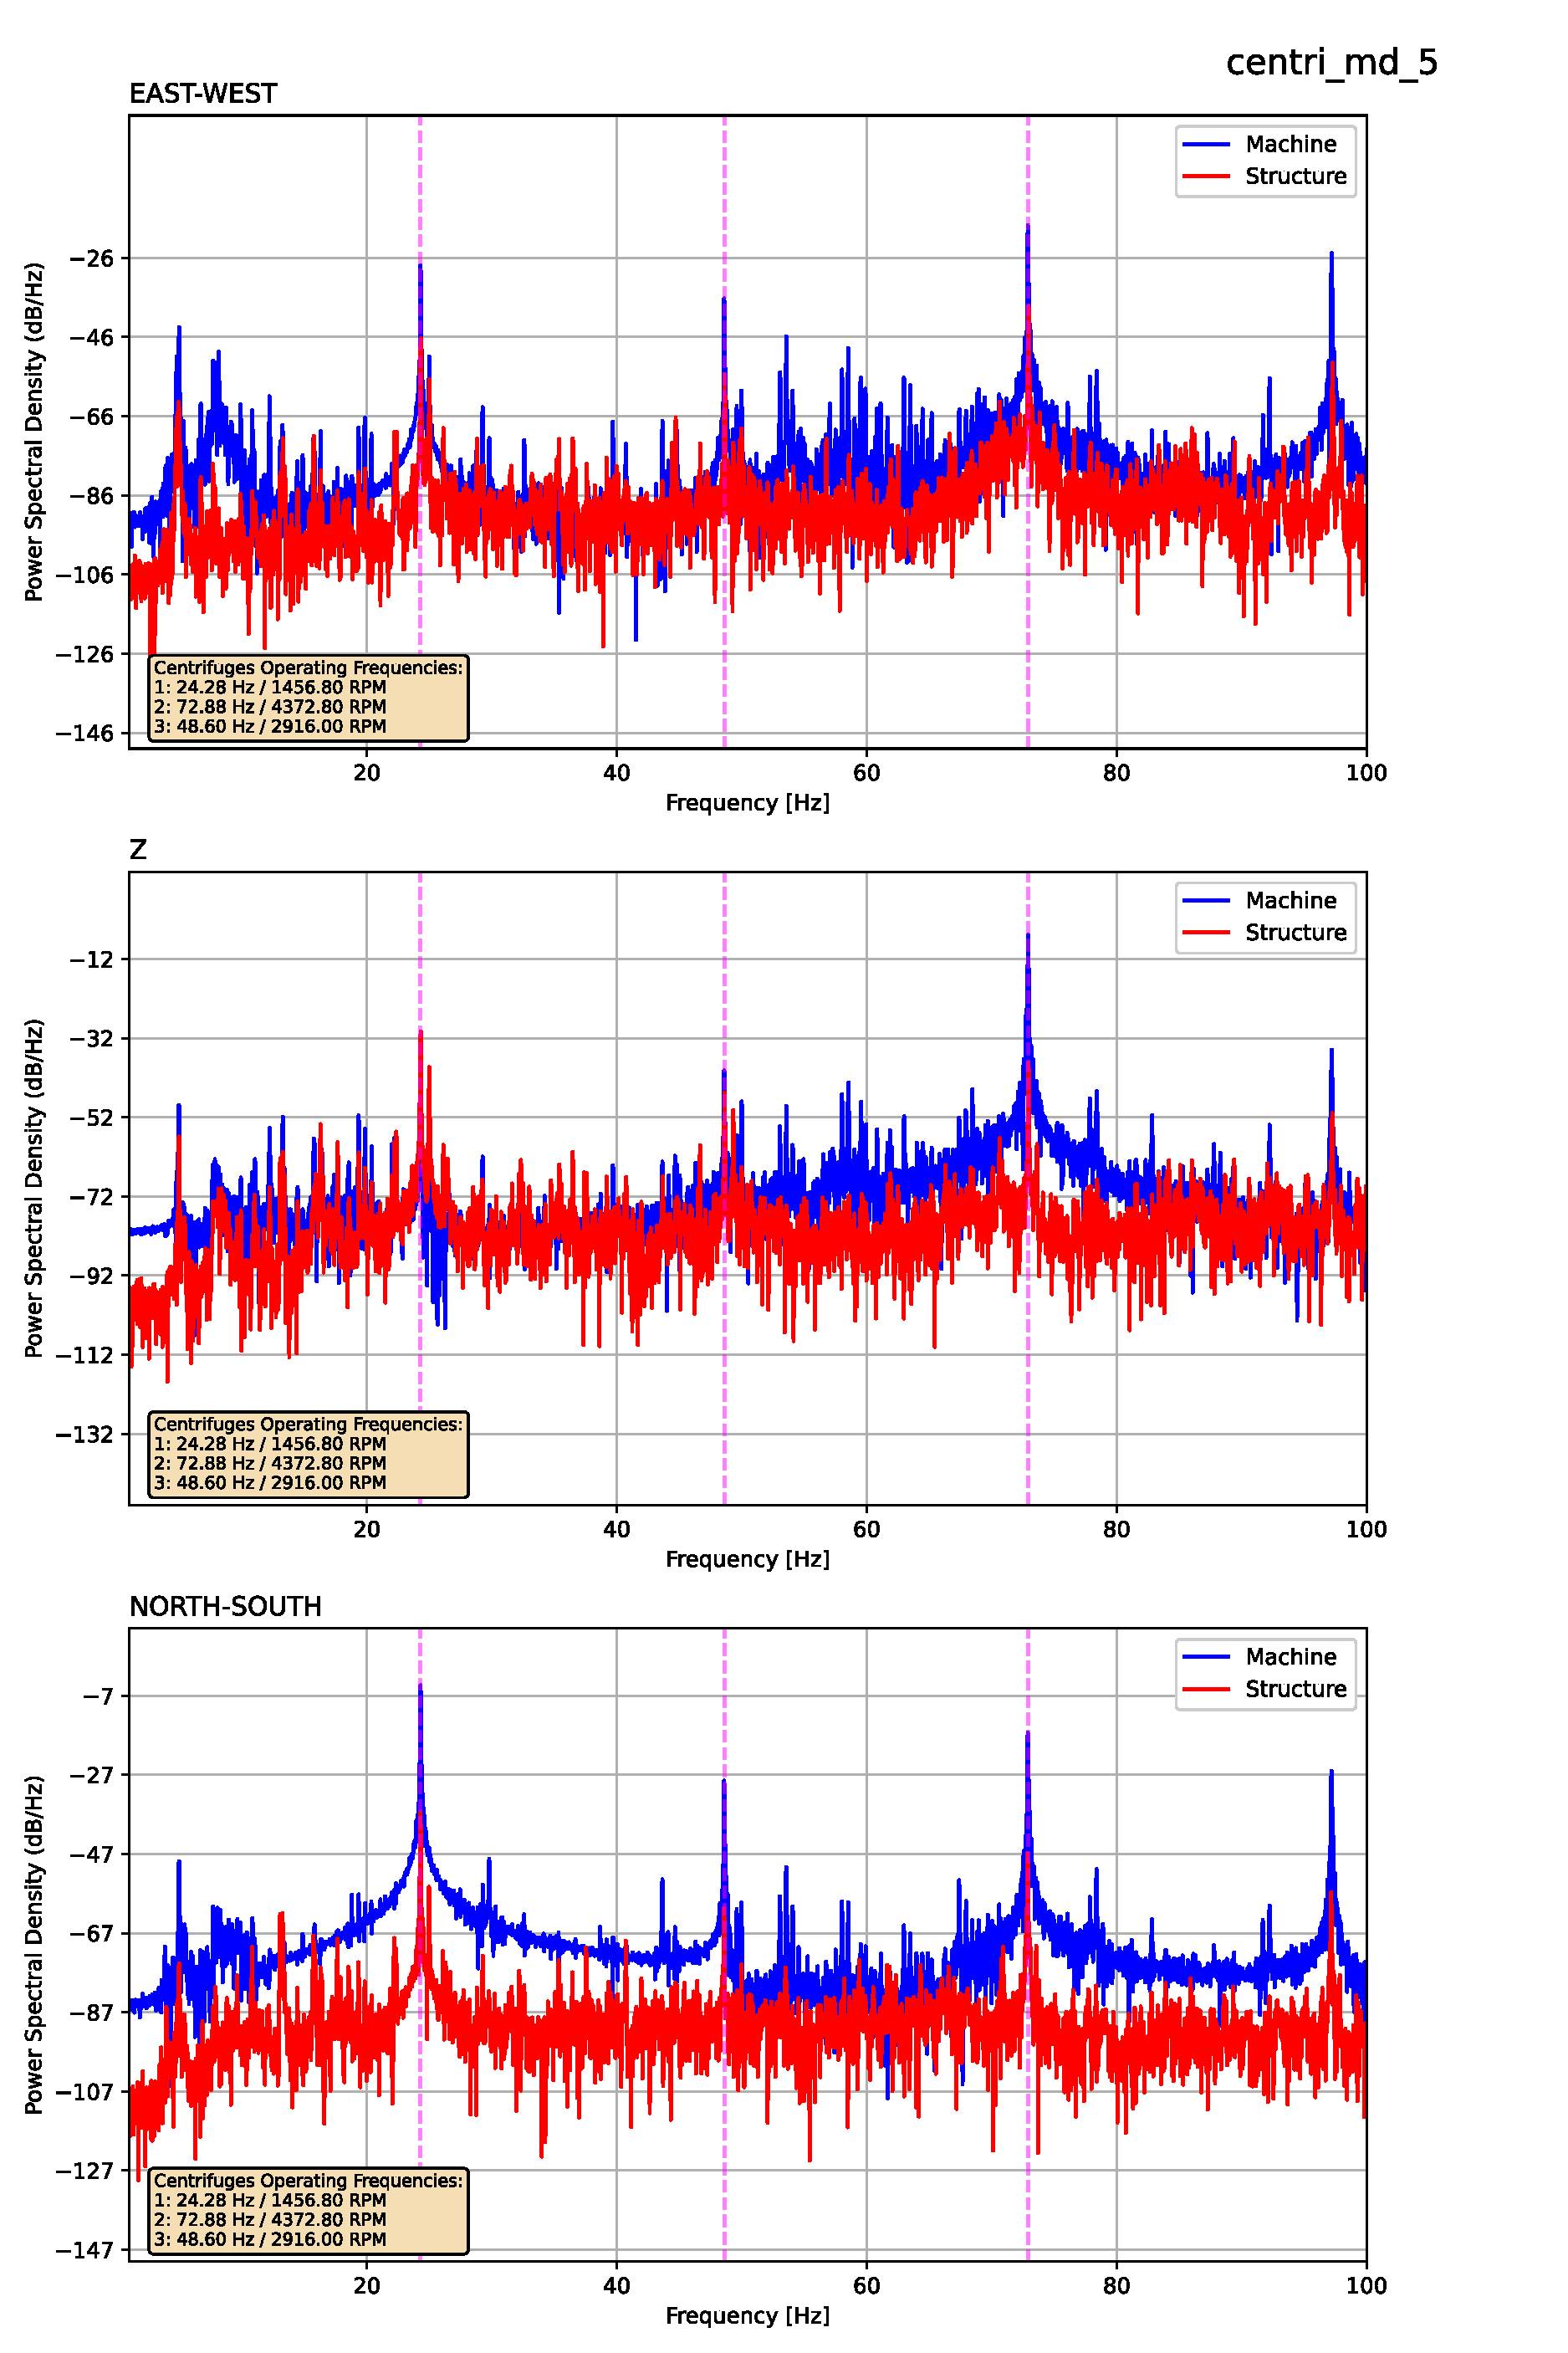
\includegraphics[width=0.3\linewidth, valign=c]{./centri_md_5_comparison.pdf} &
\includegraphics[width=0.3\linewidth, valign=c]{./centri_photos/mod5.JPG} \\
\multicolumn{2}{|p{0.6\textwidth}|}{A vibration assessment was carried out in the following centrifuges measuring acceleration above the vibration dampers and in the supporting structure (after the vibration dampers), the following frequencies were identified: [24.28 72.88 48.6 ] Hz.
} \\
\end{tabular*}
\end{center}
\newpage
\begin{center}
\begin{tabular*}{0.6\textwidth}{@{\extracolsep{\fill}}cc}
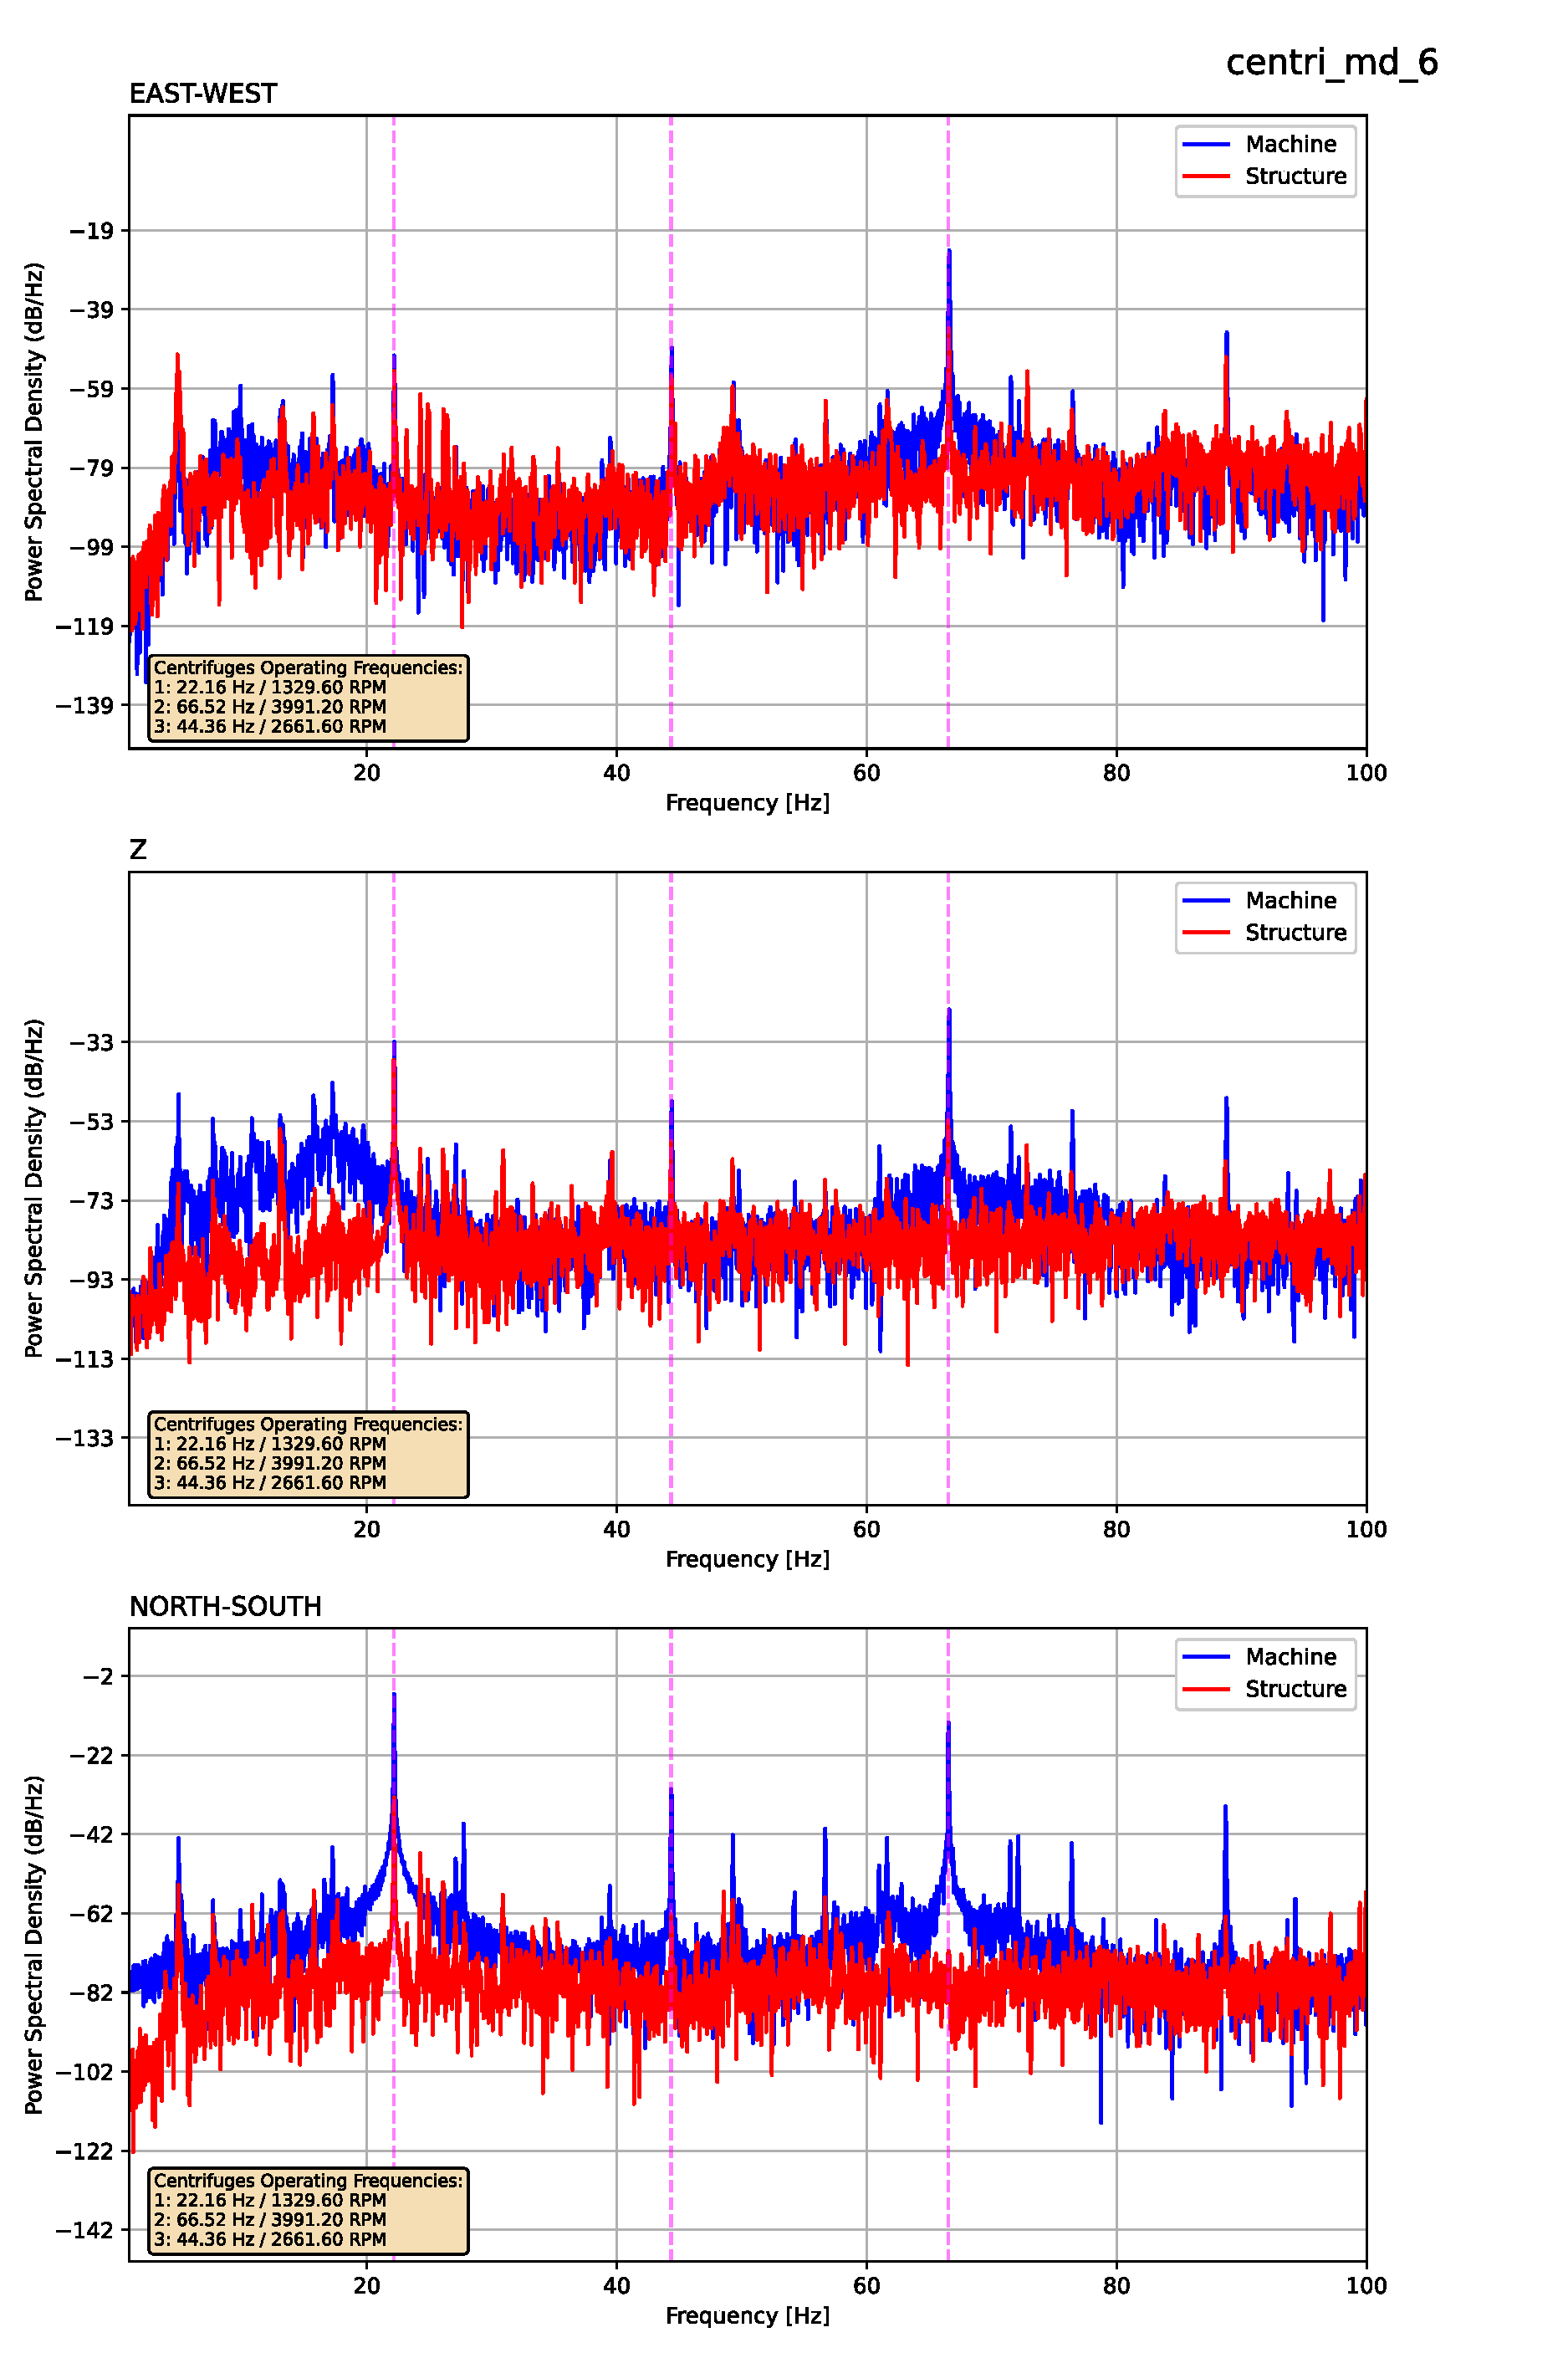
\includegraphics[width=0.3\linewidth, valign=c]{./centri_md_6_comparison.pdf} &
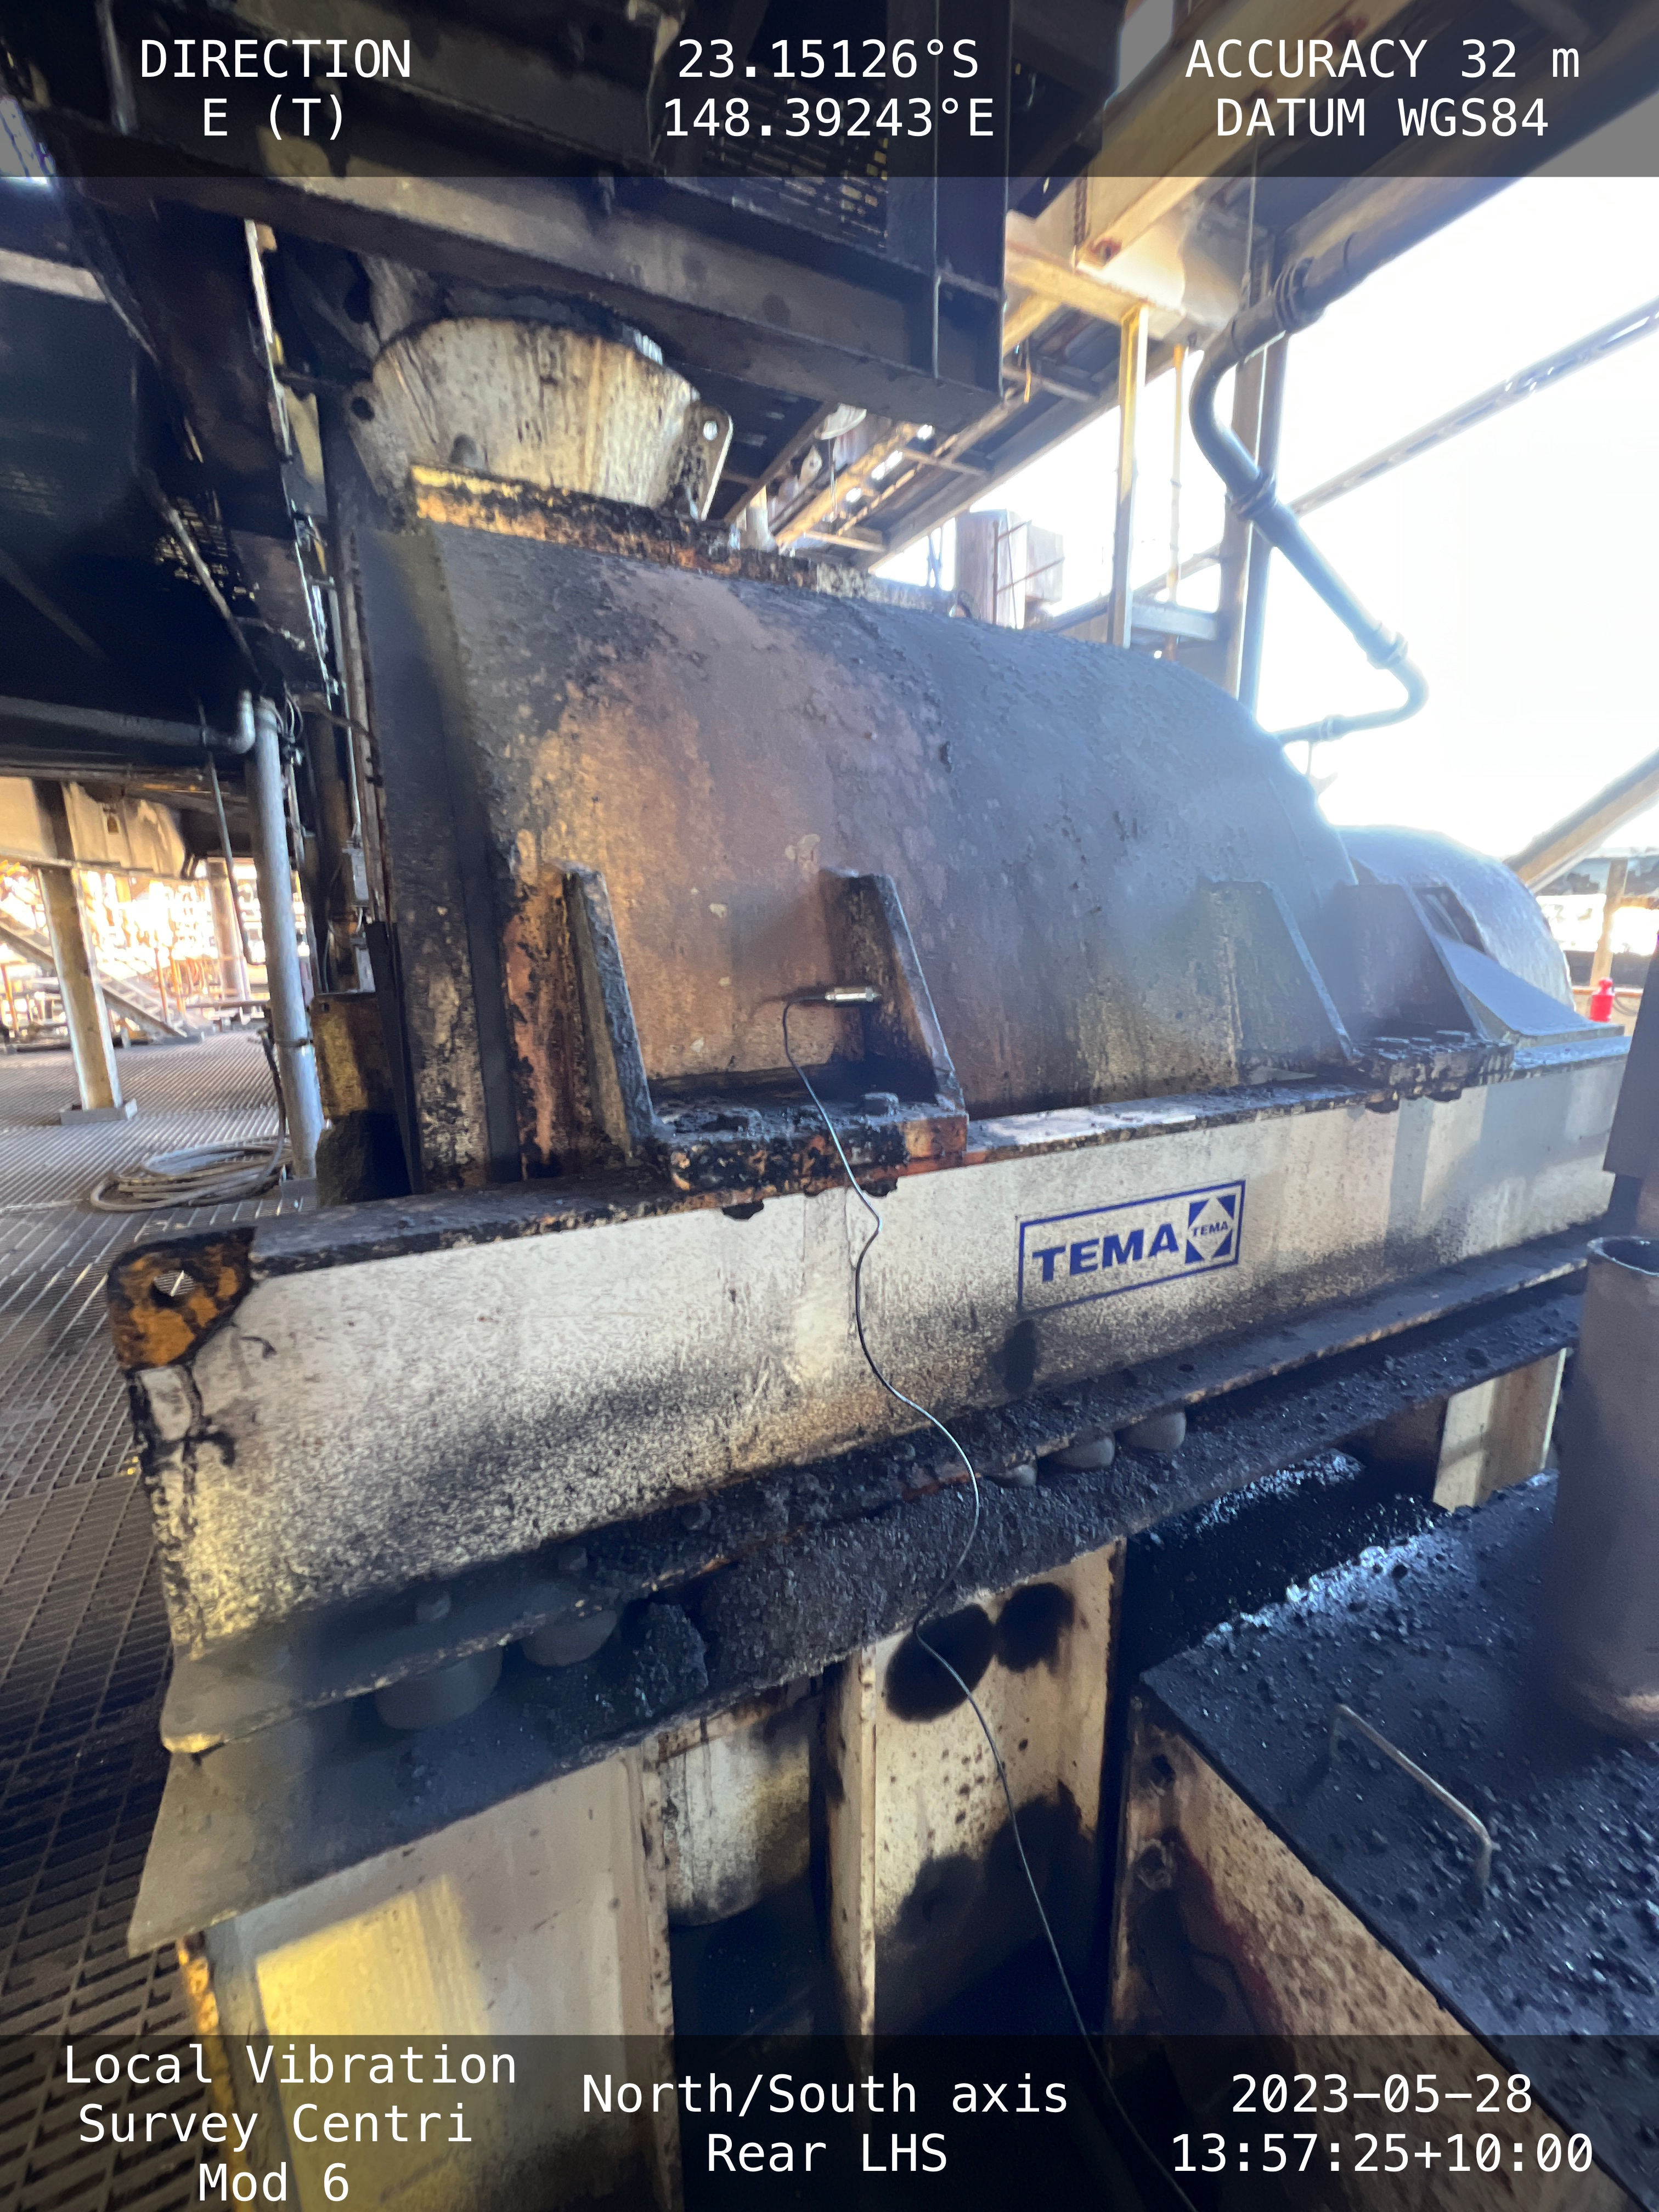
\includegraphics[width=0.3\linewidth, valign=c]{./centri_photos/mod6.JPG} \\
\multicolumn{2}{|p{0.6\textwidth}|}{A vibration assessment was carried out in the following centrifuges measuring acceleration above the vibration dampers and in the supporting structure (after the vibration dampers), the following frequencies were identified: [22.16 66.52 44.36] Hz.
} \\
\end{tabular*}
\end{center}
\newpage
\end{document}
